\begin{frame}
\frametitle{Файловая система FAT}
\begin{itemize}
  \item FAT простая и очень популярная ФС появившаяся в 1977
    \begin{itemize}
      \item Microsoft, NCR, SCP, IBM, Compaq, Digital Research, Novell;
      \item FAT расшифровывается как File Allocation Table;
      \item она неплохо работает при небольших объемах диска;
      \item не предоставляет средств обеспечения надежности;
    \end{itemize}
\end{itemize}
\end{frame}

\begin{frame}
\frametitle{Разметка диска в FAT}
\begin{figure}
  \centering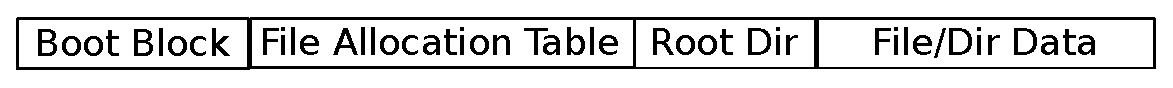
\includegraphics[width=.8\linewidth]{fat-layout}
  \caption{FAT Layout}
\end{figure}
\begin{itemize}
  \item Boot Block - содержит общую информацию (параметры диска, размер блока ФС и прочее), размер фиксирован;
  \item File Allocation Table - таблица блоков файловой системы (по одно записи на каждый блок), размер определяется при форматировании;
  \item Root Dir - содержимое корневого каталога ФС;
  \item File/Dir Data - содержимое остальных каталогов и файлов;
\end{itemize}
\end{frame}

\begin{frame}
\frametitle{File Allocation Table}
\begin{figure}
  \centering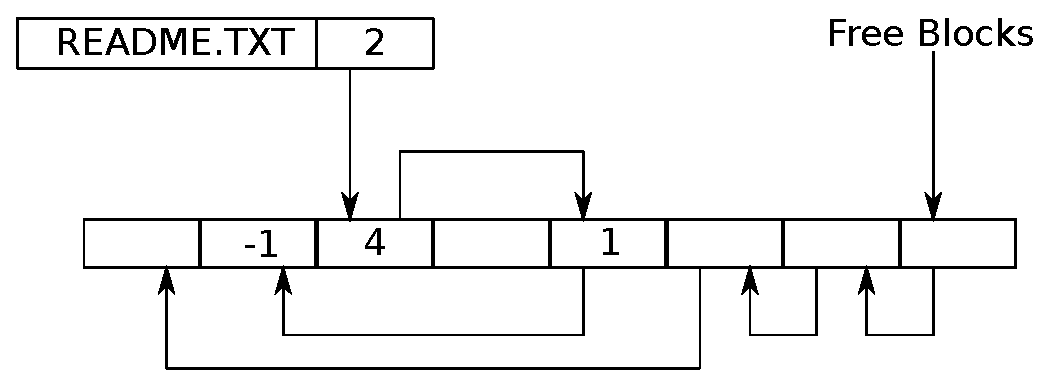
\includegraphics[width=.6\linewidth]{fat}
  \caption{File Allocation Table}
\end{figure}
\begin{itemize}
  \item Главная структура для FAT - File Allocation Table:
    \begin{itemize}
      \item File Alocation Table хранит связные списки блоков файлов/каталогов;
      \item File Allocation Table хранит номер следующего блока или маркер конца списка;
      \item зная первый блок легко получить все остальные;
    \end{itemize}
\end{itemize}
\end{frame}

\begin{frame}
\frametitle{Запись каталога}
\begin{itemize}
  \item Каталог - просто набор записей;
  \item все записи в каталоге имеют одинаковую структуру:
    \begin{itemize}
      \item 8 байт на имя + 3 байта на расширение;
      \item различные атрибуты файла (права, размер в байтах);
      \item номер первого блока файла;
    \end{itemize}
\end{itemize}
\end{frame}
